%-----------------------------------------------------------
%-----------------------------------------------------------
%	Guide d'introduction à Java et WPILib
%	Par Étienne Beaulac
%	Ultime 5528
%	Mai 2017
%-----------------------------------------------------------
%-----------------------------------------------------------


\documentclass[12pt]{report}

%Code display, avant Babel !
%\usepackage{listings, minted}

\usepackage[francais]{babel}
\usepackage[utf8]{inputenc}
\usepackage[scaled]{helvet}
\renewcommand\familydefault{\sfdefault} 
%\usepackage{libertine}
%\usepackage{libertinust1math}
\usepackage[T1]{fontenc}
%\usepackage{lmodern}
%\usepackage{avant}

% Marges
\usepackage[margin=2cm]{geometry}

%Custom font sizes
\usepackage{anyfontsize}

%Tableau en français (et non table)
%\usepackage{caption}
%\captionsetup[table]{name=Tableau}

%packages graphiques, mathématiques
\usepackage{amsfonts, amsmath, amssymb}

%Afficher des images avec includegraphics
\usepackage{graphicx}

%Image avec caption
\newcommand{\image}[2]{%

}



%Virgule pour nombres français
%\usepackage{icomma}

%Liens hypertextes
\usepackage{hyperref}
\hypersetup{
    colorlinks=true,
    linkcolor=blue,
    filecolor=magenta,      
    urlcolor=blue,
}

%Couleurs
\usepackage{xcolor}
\definecolor{ultRed}{RGB}{190,30,45}
\definecolor{ec-red}{RGB}{237,28,36}
\definecolor{ec-orange}{RGB}{255,127,39}
\definecolor{ec-yellow}{RGB}{255,242,0}
\definecolor{ec-green}{RGB}{34,177,76}
\definecolor{ec-purple}{RGB}{163,73,164}

%\usepackage{eso-pic}

%Nice code snippets
\usepackage[chapter]{minted}
\setminted[java]{%
	linenos,
	autogobble
}

%Nice frames for minted
\usepackage{tcolorbox}
\tcbuselibrary{minted, skins, xparse}
\usepackage{tikz}

%Frame for commands
\newcommand{\commande}[1]{%
\tcbox[on line, size=fbox, colframe=black, boxrule=0.75pt, tcbox raise base]{#1} %boxsep=0pt, left=5pt, right=5pt, top=8pt, bottom=8pt
}

%inline code
%\usepackage{varwidth}
%\newcommand{\code}[1]{%
%\tcbox[on line, size=fbox, colframe=gray, boxrule = 0.25pt, tcbox raise base]{\texttt{#1}} %boxsep=0pt, left=5pt, right=5pt, top=8pt, bottom=8pt
%}

%Frame for minted listings
\newtcblisting[list inside=mybox, auto counter, number within=chapter]{MyTCB}[2][]{%
	colframe=ultRed,
	title={\textsc{Code \thetcbcounter} --- #2},
	sharp corners=south,
	boxsep=3mm,
	left=0.7cm,
	listing only,
	list text={#2},
	minted language=java,
	minted options={linenos, autogobble, baselinestretch=1, tabsize=4}, #1}

%Frame for minted listings
\newtcblisting{code}[1][\linewidth]{%
	colframe=ultRed,
	sharp corners=all,
	boxsep=1mm,
	left=0.7cm,
	listing only,
	width = #1,
	minted language=java,
	minted options={linenos = false, autogobble, baselinestretch=1, tabsize=4}}


%Commande pour images inline
\newcommand{\inlinepic}[1]{%
  \begingroup\normalfont
  \includegraphics[height=1em]{#1}%\fontcharht\font`\B
  \endgroup
}

%Listings caption
\renewcommand{\listingscaption}{Extrait de code}
\renewcommand{\listoflistingscaption}{Liste des extraits de code}

%Better aligned lists
\usepackage{scrextend}

%\usepackage{multirow}
%\usepackage{tikz}
%\usepackage{pgfplots}
%\pgfplotsset{width=7cm, compat=1.13}
%\usepgfplotslibrary{fillbetween}

%\setlength{\jot}{10pt} % Modifie l'espace entre les équations d'un bloc Align

%\showboxdepth=\maxdimen
%\showboxbreadth=\maxdimen


%Indentation nul au début de paragraphe
\setlength{\parindent}{0pt}

%Espace entre les paragraphes
\setlength{\parskip}{0.5\baselineskip}


%Espace entre les notes de bas de page
\setlength{\footnotesep}{0.95\baselineskip}



%----------------------------------------------------
%----------------------------------------------------
%----------------------------------------------------
% Début du document
%----------------------------------------------------
%----------------------------------------------------
%----------------------------------------------------

\begin{document}
%
%
%----------------------------------------------------
%----------------------------------------------------
% Page titre
%----------------------------------------------------
%----------------------------------------------------
%
%
\begin{titlepage}
	\vspace*{2.5cm}
	\hspace*{-2cm}\colorbox{ultRed}{%
	{\begin{minipage}{\paperwidth}	
		{\ \\[1cm] \hspace*{2cm} {\fontsize{40}{50}\selectfont Formation Java} \\[10pt]
		\hspace*{2cm} {\Large Introduction au langage Java et à WPILib} \vspace*{1cm}}
	\end{minipage}}}\\[10pt]
	%
	\begin{minipage}{6cm}
		\raisebox{-0.1\height}{\parbox[b]{4cm}{\raggedleft {\large Étienne Beaulac\\[5pt] Ultime FRC 5528}\\[15pt] {\small Dernière modification\\ \today} }}%
		\hspace*{0.05\textwidth}%
		\raisebox{-0.5\height}{\rule{0.5pt}{6cm}}%
		\hspace*{0.32\textwidth}%
		\raisebox{-0.5\height}{
\includegraphics[trim={2.6cm 0 2.6cm 0}, clip, height=7cm]{logo_ultime.png}}%
	\end{minipage}
\end{titlepage}
\pagebreak
%
\thispagestyle{empty}
\strut
\newpage
%
% Enlever les hyperliens bleus
{\hypersetup{hidelinks}
%
\clearpage
\pagenumbering{roman}
\setcounter{page}{1}

\tableofcontents

\newpage
%
\tcblistof[\section*]{mybox}{Table des extraits de code}
\addcontentsline{toc}{chapter}{Table des extraits de code}
\newpage
%
\listoffigures
\addcontentsline{toc}{chapter}{Table des figures}
\newpage
%
\linespread{1.5}
\normalsize
\pagenumbering{arabic}
\setcounter{page}{1}
} % Fin hyperliens noirs


%----------------------------------------------------
% Ajouter fancyhf{}
%----------------------------------------------------

\part{Les bases de Java}

%----------------------------------------------------
%----------------------------------------------------
%----------------------------------------------------
% Chapitre 1 - Introduction au Java
%----------------------------------------------------
%----------------------------------------------------
%----------------------------------------------------
\chapter{Introduction au Java}
%
%
%----------------------------------------------------
% Section - Les langages de programmation
%----------------------------------------------------
%
\section{Les langages de programmation}
La programmation, en somme, est l'art de formuler ses algorithmes de manière à les faire comprendre à un ordinateur (Ada Lovelace, vers 1840\footnote{On attribue à Ada Lovelace, mathématicienne britannique, la création des premiers programmes informatiques. Ils furent conçus pour être exécutés sur la machine analytique de William Babbage, entièrement mécanique.}). Cependant, à la base, les ordinateurs ne comprennent que le binaire (Alan Turing, 1936\footnote{Alan Turing, mathématicien, cryptologue et logicien britannique, formalisa en 1936 le concept mathématique de \emph{machine de Turing}.}). Pour se simplifier la vie, les informaticiens ont créé des langages intermédiaires qui font le pont entre nous et les ordinateurs (Grace Hopper, 1951\footnote{Grace Hopper, informaticienne et \emph{rear admiral (lower half)} de l'armée américaine, conçut en 1951 \emph{A-0 System}, le premier compilateur pour ordinateur.}). Tous les langages de programmation ont le même but : vous permettre de parler à un ordinateur plus simplement qu'en binaire.
%
%
% Image - Processus de compilation
%
\begin{figure}[!htbp]
  \centering
  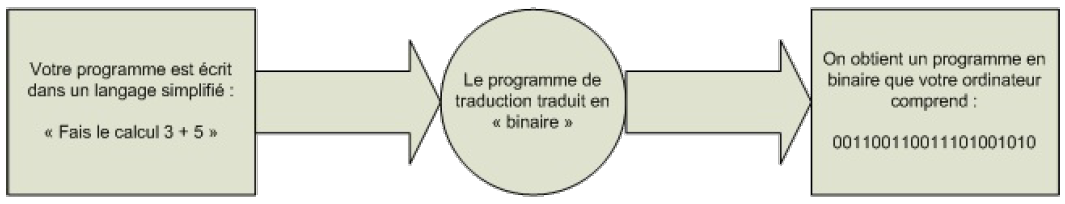
\includegraphics[width=0.9\textwidth]{compilation.png}
  \caption{Le processus de compilation.}
\end{figure}






%----------------------------------------------------
% Section - Qu'est-ce que le Java?
%----------------------------------------------------
%
\section{Qu'est-ce que le Java?}
%
%
Le langage Java a été créé , entre autres, par James Gosling, Patrick Naughton et Mike Sheridan, tous les trois employés chez \emph{Sun Microsystems} dans les années 1990. Sa première version parut en 1995. Java est maintenant propriété de \emph{Oracle Corporation}.

Java reprend une grande partie de la syntaxe du C/C++. Toutefois, les notions de pointeurs et d'héritage multiple, complexes pour les débutants, y sont absentes. Java est donc un langage presque entièrement \textbf{orienté objet}.

Le Java compte un nombre impressionnant d'utilisateurs. Une de ses forces est d'ailleurs sa portabilité. Tout programme Java, une fois compilé, peut fonctionner sur n'importe quelle machine, tant qu'une machine virtuelle Java (JRE, ou \emph{Java Runtime Environment}) y est installée.




%--------------------------------------------------------
% Chapitre - Votre premier programme 
%--------------------------------------------------------
%
\chapter{Votre premier programme}

%--------------------------------------------------------
% Section - Les environnements de développement intégré 
%--------------------------------------------------------
% TODO : Annexe A - Eclipse
%
\section{L'IDE Eclipse}
%
Pour programmer, il est préférable d'utiliser un bon environnement de développement (\textbf{IDE}, ou \emph{Integrated Development Environment}). De tels logiciels comprennent un \textbf{éditeur de texte}, un \textbf{compilateur} et un \textbf{débogueur}. Nous utiliserons l'IDE Eclipse\footnote{Pour plus d'information concernant Eclipse, consultez ...} avec l'extension WPILib fournie par FIRST.

Eclipse est disponible gratuitement sur \href{https://www.eclipse.org}{eclipse.org}. Vous devrez également vous assurer d'avoir installé une version récente du \href{http://www.oracle.com/technetwork/java/javase/downloads/index.html}{JDK} (\emph{Java Development Kit}). Les étapes d'installation sont également détaillées \href{http://wpilib.screenstepslive.com/s/4485/m/13809/l/599681-installing-eclipse-c-java}{ici}.

% Image - Interface principale de Eclipse
%
\begin{figure}[!htb]
  \centering
  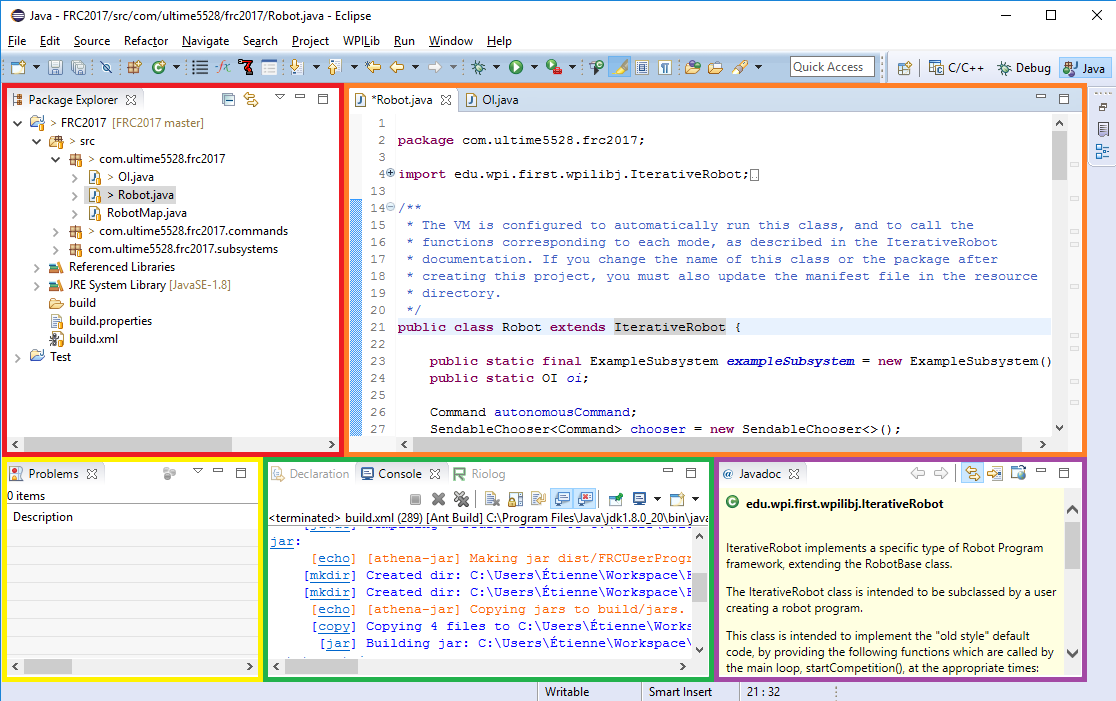
\includegraphics[width=\textwidth]{interface-eclipse.png}
  \caption{L'interface principale de Eclipse.}
\end{figure}
%
Eclipse est un logiciel ayant plusieurs fonctionnalités. On peut d'ailleurs lui en ajouter à l'aide d'extensions (\emph{plugins}), comme celle que nous utiliserons pour développer sur le roboRIO. Voici les fenêtres qui nous intéresserons le plus :

\begin{labeling}{\ Package Explorer\ }
%
\item[\colorbox{ec-red}{\emph{Package Explorer}}] Cette fenêtre regroupe tous vos projets, subdivisés en dossiers et paquetages (\emph{packages}), jusqu'aux fichiers Java.
%
\item[\colorbox{ec-orange}{Fenêtre d'édition}] Cette fenêtre affiche tous les fichiers que vous êtes en train d'éditer, vous permettant facilement de naviguer entre différents documents.
%
\item[\colorbox{ec-yellow}{\emph{Problems}}] Comme son nom l'indique, on y retrouve une liste de tous les avertissement et erreurs concernant votre code. Chaque item précise la nature de l'erreur et où elle se trouve.
%
\item[\colorbox{ec-green}{Console}] La console est un outil essentiel, c'est le premier lien entre vous et l'exécution de votre programme. Vous pourrez y afficher du texte et en insérer.
%
\item[\colorbox{ec-purple}{Javadoc}] Java a l'avantage de fournir son propre outil de documentation. Il suffit de cliquer sur un mot (classe, variable, méthode, etc.) et sa description y apparaîtra. Nous verrons plus loin comme créer ses propres entrées pour Javadoc.
\end{labeling}

Évidemment, toute l'interface est entièrement personnalisable. À vous de l'adapter comme il vous plaira!






%--------------------------------------------------------
% Section - Création du projet 
%--------------------------------------------------------
%
\section{Création du projet}
%
\begin{enumerate}
\item Dans Eclipse, créez un nouveau projet avec \commande{File > New > Java Project}. Donnez un nom à votre projet, puis cliquez sur \commande{Finish}.

\item Ajoutez une classe à votre projet : \commande{Clic droit sur votre projet > New > Class}. Donnez un nom à votre classe, cochez l'ajout de la méthode \commande{main}, puis cliquez sur \commande{Finish}.

\item Complétez le corps de la méthode avec l'exemple suivant, puis compilez et exécutez votre programme.
\end{enumerate}
%
% Code - Programme de base
%
\begin{MyTCB}{Programme de base}
public class MonPremierProgramme {

	public static void main(String[] args) {
	
		System.out.println("Hello, world");
		
	}
	
}
\end{MyTCB}
%
%
% Image - Compiler/Exécuter avec Eclipe
\begin{figure}[!htb]
	\centering
	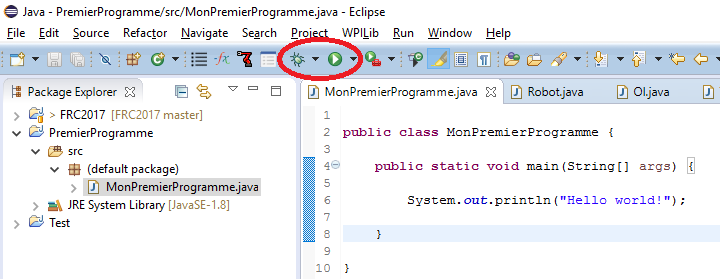
\includegraphics[width=\textwidth]{compilation-eclipse.png}
	\caption{Compiler, exécuter et déboguer un progamme avec Eclipse.}
\end{figure}
%
Le bouton \inlinepic{debug-btn-eclipse.png} vous permet de lancer votre programme en mode débogage. La flèche verte \inlinepic{execute-btn-eclipse.png}, quant à elle, compile et exécute. Après avoir cliqué dessus, vous devriez voir apparaître du texte dans votre console.
%
% Image - Écriture console
%
\begin{figure}[!ht]
	\centering
	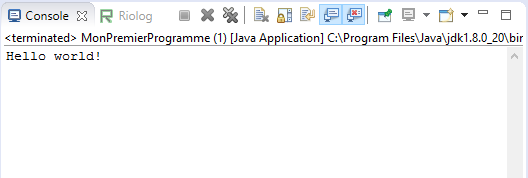
\includegraphics[scale=1]{ecriture-console.png}
	\caption{Écriture dans la console.}
\end{figure}

Félicitations, vous venez d'exécuter votre premier programme! Décortiquons en détails ce qu'il se passe à l'intérieur.






%--------------------------------------------------------
% Section - Instructions
%--------------------------------------------------------
%
\section{Les instructions}
En Java, une \textbf{instruction} est une commande effectuant une certaine action. On écrit une instruction par ligne, et chacune se termine toujours par un \textbf{point-virgule} (\ {;}\ ). Pour l'instant, votre programme ne contient qu'une instruction : 
\begin{code}
System.out.println("Hello, world!");
\end{code}
Vos instructions sont écrites dans la méthode \texttt{\bfseries main}. En Java, tous les programmes ont une méthode \texttt{main}. Il s'agit, en quelque sorte, du point d'entrée du programme.





%--------------------------------------------------------
% Section - Les chaînes de caractères
%--------------------------------------------------------
%
\section{Les chaînes de caractères}
%
Le rôle de votre programme est d'afficher du texte dans la console. Vous avez sûrement remarqué que le texte à afficher est encadré de guillemets anglais ("..."), mais qu'ils n'apparaissent pas dans la console. Ils sont essentiels pour que le compilateur fasse la différence entre du code et du texte. On les appelle des \textbf{chaînes de caractères}, ou \emph{\bfseries String} en anglais. Essayer de modifier le texte entre les guillemets et d'exécuter votre programme : vous constaterez que la chaîne de caractères affichée dans la console s'est modifiée!

On peut joindre plusieurs chaînes de caractères ensemble avec l'opérateur \commande{+}. Cette opération s'appelle la \textbf{concaténation}. On peut donc écrire :%
\begin{code}
System.out.println("Bonjour " + "à tous" + " et à toutes" + "!");
\end{code} 





%--------------------------------------------------------
% Section - La méthode println
%--------------------------------------------------------
%
\section{La méthode \texttt{println}}
%
En Java, une \textbf{méthode} est une instruction qui réalise une opération prédéfinie. On utilise une méthode en écrivant son nom suivi d'une paire de parenthèses. Certaines méthodes ont besoin de paramètres pour effectuer leur travail. C'est le cas de la méthode \texttt{System.out.println}, qui demande un \emph{String} en paramètre. Elle s'occupe ensuite de l'afficher sur la console.




%--------------------------------------------------------
% Section - Indentation
%--------------------------------------------------------
%
\section{L'indentation}
%
Dans l'exemple précédent, vous pouvez constater qu'à chaque fois que des accolades ({...}) sont ouvertes, on ajoute de l'espace au code qui se situe à l'intérieur. C'est ce que l'on appelle l'\textbf{indentation} du code. C'est essentiel pour rendre le code clair et facile à modifier. Pour indenter son code, on ajoute une tabulation (touche \commande{Tab $\rightleftarrows$}) pour chaque paire ouverte d'accolades. Eclipse s'en occupe automatiquement la plupart du temps.







%--------------------------------------------------------
% Section - Les commentaires
%--------------------------------------------------------
%
\section{Les commentaires}
%
%
%
\subsection{Les commentaires standards}
%
%
Lors de l'écriture, il est possible de spécifier au compilateur de ne pas compiler certaines parties du code. C'est ce qu'on appelle les \textbf{commentaires}. Ils permettent de spécifier l'utilité des variables, des méthodes, des classes, etc. Il est crucial d'en ajouter, surtout lors d'un projet en collaboration avec plusieurs personnes!

%
% Code - Premier programme avec commentaires standards
%
\begin{MyTCB}{Programme de base avec commentaires}
/* 
 * La classe suivante affiche un message
 * dans la console.
 */
public class MonPremierProgramme {

	/*  Fonction principale
		du programme.		*/
	public static void main(String[] args) {
	
		//Début du programme
		
		System.out.println("Hello, world"); //Affichage du message
		
	}
	
}
\end{MyTCB}
%
%
Les plus courants sont les \textbf{commentaires en fin de ligne}. Ils débutent par deux barres obliques \mbox{\commande{//}.} Ils informent le compilateur d'ignorer tout le reste de la ligne. Ils sont souvent courts et précis. On les utilise pour mettre en contexte une instruction ou en début de section.

Pour de longs commentaires, on utilise les \textbf{commentaires en blocs}. Ils débutent par \commande{/*} et se terminent par \commande{*/}. Le compilateur ignore alors tout ce qui se trouve entre ces deux balises, un peu comme des parenthèses. On les utilise, entre autres, en entête de fichier, pour spécifier le rôler du fichier (ou de la classe), les noms des auteurs et les dates de création et de modification.

Il est important de mettre des commentaires, mais il ne faut pas en abuser (comme dans l'exemple précédent). Il suffit de trouver le juste équilibre entre clarté et concision. Il est également essentiel de mettre en contexte l'instruction.

Bon commentaire :
\begin{code}
age += 1; // L'utilisateur vieillit d'un an.
\end{code}

Mauvais commentaire :
\begin{code}
age += 1; // Ajout de 1 à la variable age.
\end{code}


% Commentaires Javadoc
%
\subsection{Les commentaires Javadoc}
%
%
Ces commentaires spéciaux sont propres au Java. Ils permettent de créer une documentation accessible pour votre projet. Ils sont très semblables aux commentaires en blocs : il suffit de les faire débuter avec deux étoiles \commande{/**}. Vous aurez donc accès au contenu de votre commentaire partout dans votre projet, sans devoir ouvrir à nouveau le fichier d'origine!
%
% Code : Commentaire Javadoc
%
\begin{MyTCB}{Ajout de commentaires Javadoc}
/**
 * Ceci est un commentaire Javadoc!
 * @author Etienne
 *
 */
public class MonPremierProgramme { ... }
\end{MyTCB}
%
%
\begin{figure}[!ht]
	\centering
	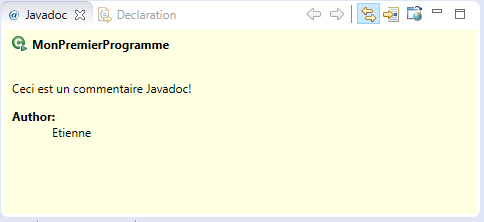
\includegraphics[scale=1]{javadoc-eclipse.png}
	\caption{Visualisation de la Javadoc dans Eclipse}
\end{figure}
%
%
La Javadoc possède plusieurs attributs spéciaux débutant par un arrobe \commande{@}. Les exemples de ce guide feront appel aux trois attributs suivants.

\begin{labeling}{@author\ }

\item[\textbf{@author}] On l'utilise dans l'entête d'une classe pour en spécifier l'auteur.
\item[\textbf{@param}] Dans l'entête de méthodes, il précise le rôle de chaque paramètre.
\item[\textbf{@return}] Également dans l'entête de méthodes, il précise la valeur de retour.

\end{labeling}
%





\end{document}













\begin{tcolorbox}[adjusted title=Titre 1]
Allo !
\end{tcolorbox}
%
\begin{tcblisting}{}
	Test!
\end{tcblisting}





%Enlever les trop grands espaces entre les titres
\usepackage{titlesec}

\titleformat{\chapter}[display]   
{\normalfont\huge\bfseries}{\chaptertitlename\ \thechapter}{20pt}{\Huge}   
\titlespacing*{\chapter}{0pt}{\parskip}{-\parskip}
\titlespacing{\section}{0pt}{\parskip}{-\parskip}
\titlespacing{\subsection}{0pt}{\parskip}{-\parskip}
\titlespacing{\subsubsection}{0pt}{\parskip}{-\parskip}





